\documentclass[12pt]{article}
\usepackage[english]{babel}
\usepackage[margin=0.90in]{geometry}
\usepackage{amsmath}
\usepackage{amssymb}
\usepackage{siunitx}
\usepackage{algorithm}
\usepackage[noend]{algpseudocode}
\usepackage[utf8]{inputenc}
\usepackage{graphicx}
\usepackage{listings}
\usepackage{color}
\usepackage{hyperref}
\usepackage{cite}
%\usepackage{textcomp,uiosloforside}
\numberwithin{figure}{section}
\numberwithin{table}{section}

\definecolor{mygreen}{rgb}{0,0.6,0}
\definecolor{mymauve}{rgb}{0.58,0,0.82}
\definecolor{mygray}{rgb}{0.97,0.97,0.97}
  
\lstset{
  language=C++,
  basicstyle=\footnotesize,
  commentstyle=\color{mygreen},
  keywordstyle=\color{blue},
  stringstyle=\color{mymauve},
  tabsize=4
}

\newcommand{\dydx}{\frac{\partial\psi}{\partial x}}
\newcommand{\dydy}{\frac{\partial\psi}{\partial y}}
\newcommand{\dyydxx}{\frac{\partial^2\psi}{\partial x^2}}
\newcommand{\dyydyy}{\frac{\partial^2\psi}{\partial y^2}}
\newcommand{\dydt}{\frac{\partial\zeta}{\partial t}}
\newcommand{\dyydtt}{\frac{\partial^2\zeta}{\partial t^2}}
\newcommand{\Ixyt}{|_{x,y}^{t}}
\newcommand{\IIxyt}{\Bigr|_{x,y}^{t}}
\newcommand{\Ixytp}{|_{x,y}^{t\pm\Delta t}}
\newcommand{\Ixytm}{|_{x,y}^{t-\Delta t}}
\newcommand{\Ixpyt}{|_{x\pm\Delta x,y}^{t}}
\newcommand{\Ixmyt}{|_{x-\Delta x,y}^{t}}
\newcommand{\Ixypt}{|_{x,y\pm\Delta y}^{t}}
\newcommand{\Ixymt}{|_{x,y-\Delta y}^{t}}
\newcommand{\Ijkn}{|_{j,k}^{n}}
\newcommand{\Ijknp}{|_{j,k}^{n+1}}
\newcommand{\IIjknp}{\Bigr|_{j,k}^{n+1}}
\newcommand{\Ijpkn}{|_{j+1,k}^{n}}
\newcommand{\Ijmkn}{|_{j-1,k}^{n}}

\begin{document}
\begin{titlepage}
\title{Project 5 - FYS4150}
\author{Oda Langrekken, Trude Hjelmeland and Jostein Brændshøi}
\date{
    Department of Physics\\%
    University of Oslo\\[2ex]%
    \today
}
\clearpage
\maketitle
\thispagestyle{empty}

\begin{abstract}
\noindent We solve the barotropic Rossby wave equation in both one and two spatial dimensions by disrectizing the equations using finite difference methods. The vorticity is advanced in time using a Forward-Euler scheme and a leapfrog scheme. Then, at every time step, we solve the Poisson equation using the Thomas algorithm (1D) and the iterative Jacobi method (2D). We discover that the leapfrog scheme is by far superior to the Forward-Euler scheme when it comes to stability truncation error. Comparing with our analytical predictions, we also discover that there is great correspondence between the analytical the numerical solutions in one spatial dimension. The two-dimensional (+ time) solution does also behave as we expected.\\
\end{abstract}
\vspace{2.00cm}


\noindent The address \url{https://github.com/jostbr/FYS4150-Projects/tree/master/Project5} on Git-Hub is associated with this project. Here one can find all code used in the project. This includes C++ source files containing the core of the project, but also a Python plotting script for result visualization. There are also available benchmark results from running the code as well as \LaTeX \ source for this PDF. In addition some animations (generated with the python script) are uploaded to streamable that are associated with this project and the specifics links are provided below in the report when relevant.

\end{titlepage}
\pagebreak

\tableofcontents
\pagebreak

% ======== Indicate new section
% -------- Indicate new subsection

% ========================================================================================
% ========================================================================================
\section{Introduction} \label{sec:intro}
Several physical processes are modeled as partial differential equations, with the wave equation and the diffusion equation as some of the more well-known examples. These are equations involve multiple independent variables and partial derivatives of an unknown function with respect to these variables. As the reader can probably imagine (or has experienced themselves) the analytical solution to these problems are often hard, or in fact impossible, to find. The authors of this report were actually unable to find an analytical solution to our partial differential equation in two spatial dimensions. Luckily, we were able to solve the equations numerically.\\
%Tror det heter spatial ikke space.. 

\noindent We will in this project consider an important partial differential equation in the field of geophysical fluid dynamics. We have modeled the motion of Rossby waves, which are huge waves whose motion is largely due to the rotation of our planet, in particular due to the gradient of the planetary vorticity. Rossby waves exists in both the atmosphere and the oceans. These waves have massive wavelengths and can stretch for hundreds of kilometers in the horizontal direction, and are always moving towards the west. Due to their very small vertical movement, one relies one satellite radar to observe the waves, as they are undetectable by the naked eye (some beautiful satellite pictures with corresponding Hovmuller diagrams for oceanic Rossby waves can be found at 
\url{https://pdfs.semanticscholar.org/ade1/1c28490ee98a57027ccc3dec5d57419a8c98.pdf}).\\

\noindent The motion of Rossby waves is modeled by the barotropic Rossby wave equation
\begin{equation}
\frac{\partial}{\partial x}\nabla_H^2\psi +\beta\frac{\partial \psi}{\partial x}=0
\end{equation}

\noindent which is a linear third order partial differential equation. To solve for the motion of the waves, we rewrite this equation into two coupled PDE's and discretize the equations, then advance it in time using finite difference methods. In one dimension the problem then reduces to solving the Poisson equation, albeit at every time step, which we achieve using the Thomas algorithm from linear algebra. In two dimensions the iterative Jacobi solver is used to solve the Poisson equation.\\

\noindent We would also like to mention briefly that this project was also used to gain familiarity with class inheritance in C++. Having to implement several different solvers all related to each other presented a good opportunity to have a look at how one implements class inheritance in C++.\\


\noindent We will start our report by introducing the theory used for this project, starting by discussing some general properties of wave and then moving on to Rossby waves. We also solve the one-dimensional Rossby equation analytically for two different domains. Next we proceed to discuss the methods we have used to solve the equations numerically, with special emphasis on finite difference methods emerging from Taylor series. Finally our results are presented and discussed, before we offer some concluding remarks about what we have achieved by working with this project.\\    

%====================================================================================
%====================================================================================
\section{Theory} \label{sec:theory}

%-----------------------------------------------------------------------------------
\subsection{General waves}
\label{generalWaves}
%What is a wave? 
A wave is a disturbance that travels trough a medium where there is little to no mass transport, but through local displacements of e.g. fluid parcels, information is transported from one location to another. We do not here consider electromagnetic waves. \\   

%Explain phase speed, group velocity., dispersion (wave number and wave frequency), general wave solution (Acos ...). 

\noindent A wave equation describes how a wave propagates in a medium over time and the mathematical form of these equations varies depending on the type of wave we are describing. We will investigate waves that move trough our atmosphere and oceans. One of the most simple wave equations describes a plane wave and its wave solution usually takes the form (in one spatial dimension):

\begin{equation}
	%\psi = A cos(kx - \omega t)
    \psi (x, t) = A e^{i(kx -\omega t)}
    \label{GeneralWave}
\end{equation}


\noindent Here $\psi$ is the wavefunction, $A$ is the maximum amplitude, $\omega$ is the angular frequency and $k$ is the wave number defined as $k=\frac{2\pi}{\lambda}$ where $\lambda$ is the wavelength. The exponential term can be related to sine and cosine terms through Euler's formula. We shall see below that this plane wave appears as an analytical solution in one of the cases we study.\\

\noindent There are two velocities associated with waves, namely the group velocity and the phase velocity \cite{fluid_dynamics_notes}. The phase velocity is defined as

\begin{equation}
	v_p = \frac{\omega}{k}
    \label{PhaseVelocity}
\end{equation}

\noindent which describes the speed at which e.g. crests and troughs move. The group velocity is defined as

\begin{equation}
	v_g = \frac{\partial \omega}{\partial k}
    \label{GroupVelocity}
\end{equation}

\noindent and is related to the energy transfer supported by the wave. Both of these speeds can be found through the dispersion relation $\omega(k)$ as shall be seen for our specific cases later. \\



%-----------------------------------------------------------------------------------
\subsection{Rossby waves} \label{sec:Rossby}


\noindent Rossby waves are a natural phenomena in both our atmosphere and oceans. They are known as planetary waves since they are largely caused by the rotation of our planet and also due to their length scale of hundreds to thousands of kilometers. \\ 

%Atmospheric Rossby waves on Earth are giant meanders in high-altitude winds that have a major influence on weather. These waves are associated with pressure systems and the jet stream.

\noindent Newtons law of motion describes the motion of an object in an inertial, non accelerating, frame of reference. As the motion we wish to describe in this project finds place in the atmosphere and oceans of our rotating planet, we need to transform Newtons law in to a rotating frame of reference. Here forces like the Coriolis force and centrifugal force come into play. For the purpose of this project the Coriolis force, $F_c$, is the actor of importance, and this force is proportional to the mass of the object, $m$, which it acts upon and the rotational rate, $\Omega$, of our planet. The Coriolis force is defined as:

\begin{equation}
		\mathbf{F_C} = - 2 m \mathbf{\Omega} \times  \mathbf{v} 
\end{equation}

\noindent Here $\mathbf{v}$ is the velocity with respect to the rotating system and $\mathbf{\Omega}$  is the angular velocity with magnitude equal to the rotational rate, $\Omega$, and direction along the rotational axis of the rotating reference frame. The Coriolis force is a consequence of inertia in the system and the Coriolis acceleration is negative in the southern hemisphere and positive in the northern hemisphere. This means that a fluid parcel will experience a spin (vorticity), that varies when it moves towards different latitudes as we will see when we define the Coriolis parameter in equation \eqref{CorParam} below.   \\


\noindent The Coriolis effect is the effect added by the Coriolis acceleration and can be expressed through the Coriolis parameter, $f$, as \cite{pro5}:

\begin{equation}
		f = 2 \pi \Omega \sin(\theta)
        \label{CorParam}
\end{equation}

\noindent Here $\Omega$ is the rotational rate of the Earth, given as $\Omega = \frac{2\pi}{day}$, and $\theta$ is the latitude. Thus the latter term in equation \eqref{CorParam} expresses the latitude dependence of the planetary vorticity caused by the Coriolis acceleration as mentioned above. \\

\noindent The relative vorticity, $\zeta$, of a fluid expresses the rotation of a fluid parcel and, in the context of examining Rossby waves, is governed by the equation:

\begin{equation}
	\frac{\partial}{\partial t}\zeta + \beta \frac{\partial}{\partial x} \psi = 0
    \label{Vorticity}
\end{equation}

\noindent where $\psi$ is the streamfunction (related to pressure and thus e.g. sea-sruface-height) and $\beta$ emerges as a consequence of the $\beta$-plane approximation we will use. In this approximation we approximate the Coriolis parameter, $f$, as a linear function centered around the latitude $\theta_0$:     

\begin{equation}
	f \sim f_0 + \beta y
\end{equation}

\noindent where $f_0$ is defined as $2 \Omega \sin(\theta_0)$, $\beta = \frac{2 \Omega \cos(\theta_0)}{R_E}$, $y = R_E(\theta - \theta_0)$ and $R_E$ is the Earth's radius. \\ 


\noindent In this project we will look at motion in the $xy$-plane, neglecting the curvature of the Earth, and the corresponding velocities are determined by the streamfunction, $\psi$, through the relations (from geostrophy)\cite{fluid_dynamics_notes}:

\begin{equation}
	u = - \frac{\partial}{\partial y} \psi, \hspace{3cm} v = \frac{\partial}{\partial x} \psi
    \label{Velocity}
\end{equation}

\noindent Here $u$ is velocity in the $x$-direction, east-west, and $v$ is the velocity in the $y$-direction, north-south. The vorticity is defined through the velocities as:

\begin{equation}
	\zeta = \frac{\partial}{\partial x} v - \frac{\partial}{\partial y} u \label{eq:zeta_definition}
\end{equation}

\noindent which comes from considering the full curl of the velocity field $\mathbf{u}(x,y,t)=(u,v)$. Examining $\nabla\times\mathbf{u}$ one may see that $\zeta$ as written in \eqref{eq:zeta_definition} is in fact the $z$-component of the full curl of the velocity, i.e. $\zeta=\mathbf{k}\cdot(\nabla\times\mathbf{u})$ (in 2D flows, the curl is zero in both the $x$- and $y$-direction). And by utilizing the definitions of the velocities u and v as given in equation \eqref{Velocity} we find that the vorticity is the Laplacian of the streamfunction:

\begin{equation}
	\zeta = \nabla_H^2 \psi 
\end{equation}

\noindent where the $H$ denotes for the horizontal Laplacian. Thus the vorticity can be written in terms of just on variable, namely $\psi$, leading us to the Rossby barotropic wave equation:

\begin{equation}
	\frac{\partial}{\partial t} \nabla_H^2 \psi + \beta \frac{\partial}{\partial x} \psi = 0
    \label{Rossby}
\end{equation}

\noindent Here barotropic means depth invariant flow. In this project we will look at solutions to equation \eqref{Rossby} in both a periodic and closed domain. A periodic domain means that the wave solution is the same at both boundaries, which can be visualized as the atmosphere wrapping around the Earth. A closed domain means that the wave solution needs to be 0 at the boundaries, which can be visualized as impenetrable walls that wraps around our continents. The latter boundary condition is motivated by the fact that it is reasonable to reuqire no flow trhough the walls of the domain (in fact from the relations \eqref{Velocity} this would only seem to require $\psi$ to be some constant, but we put this constant to zero). \\

\noindent We will for simplicity in the rest of this report use the shorthand notation for the derivatives (or the ones used above):

\begin{equation*}
	\partial_t = \frac{\partial}{\partial t}, \hspace{1cm} \partial_x = \frac{\partial}{\partial x}, \hspace{1cm} \partial_y = \frac{\partial}{\partial y},
\end{equation*}

\begin{equation*}
	\partial_{xx} = \frac{\partial^2}{\partial x^2}, \hspace{1cm} \partial_{yy} = \frac{\partial^2}{\partial y^2}
\end{equation*}










%-----------------------------------------------------------------------------------

\subsection{Analytic solution to Rossby equation in periodic domain} \label{sec:analytical_periodic}
\noindent To study the Rossby equation further, let us consider the vorticity equation \eqref{Rossby} in 1-dimension in a periodic domain. We let our domain be defined by $x\in [0, L]$ in the east-west direction. A suitable streamfunction has the form \cite{pro5}  
\begin{equation}
\label{eq:wave_periodic}
\psi = A\cos\left(\frac{2n\pi x}{L}-\omega t\right)
\end{equation}
where $n$ is an integer ($n=1,2,\dots$), $A$ is the amplitude of the wave and $\omega$ is the wave angular frequency.\\ 
\noindent For \eqref{eq:wave_periodic} to be a solution in the periodic domain, we require $\psi(0,t)=\psi(L,t)$. Let us check if this requirement is met in our case
\begin{align*}
\psi(0,t)&= A\cos\left(0-\omega t\right) = A\cos\left(-\omega t\right)\\
\psi(L,t) &= A\cos\left(\frac{2n\pi L}{L}-\omega t\right)\\
&= A\left[\cos(2n\pi)\cos(-\omega t)-\sin(2n\pi)\sin(-wt) \right]\\
&=A\cos(-\omega t)
\end{align*}
where we have used $\cos(u+v)=\cos(u)\cos(v)-\sin(u)\sin(v)$ and the fact that $\cos(2n\pi)=1$ and $\sin(2n\pi)=0$ for all $n\in\mathbb{Z}$ \cite{MathMethods}. Thus $\psi(0,t)=\psi(L,t)$ and \ref{eq:wave_periodic} does indeed satisfy the periodic boundary conditions.\\

\noindent Our streamfunction \eqref{eq:wave_periodic} should also satisfy the vorticity equation \eqref{Rossby}.  Let us calculate the necessary derivatives:
\begin{equation}
\label{eq:y_velocity}
v=\partial_x\psi=-\frac{2n\pi A}{L}\sin\left(\frac{2n\pi x}{L}-\omega t\right)
\end{equation}
\begin{equation}
\label{eq:dv/dx}
\partial_x v = -\frac{(2n\pi)^2A}{L^2}\cos\left(\frac{2n\pi x}{L}-\omega t\right)
\end{equation}
\begin{equation}
\label{eq:dtdv/dx}
\partial_t \partial_x v = -\frac{(2n\pi)^2A\omega}{L^2}\sin\left(\frac{2n\pi x}{L}-\omega t\right)
\end{equation}
Inserting \ref{eq:y_velocity} and \eqref{eq:dtdv/dx} into \eqref{Rossby}, we find
\begin{equation}
 -\frac{(2n\pi)^2A\omega}{L^2}\sin\left(\frac{2n\pi x}{L}-\omega t\right)-\beta\frac{2n\pi A}{L}\sin\left(\frac{2n\pi x}{L}-\omega t\right)=0 
\end{equation}
which puts the following requirement on the wave frequency $\omega$
\begin{equation}
\label{eq:omega_periodic}
\omega = -\frac{\beta L}{2n\pi}
\end{equation}
which is known as the wave dispersion relation.\\
\noindent Using the wave dispersion relation, we can calculate the phase speed \eqref{PhaseVelocity} 
\begin{equation}
\label{eq:phase_speed_periodic}
v_p = \frac{\omega L}{2n\pi} = -\frac{\beta L^2}{(2n\pi)^2}
\end{equation}
The phase speed is negative, so the wave is moving in the negative x-direction, i.e. towards the west.\\

% ------------------------------------------------------------------------------

\subsection{Analytic solution to the Rossby equation with solid boundaries} \label{sec:analytical_bounded}
\noindent We will now find an analytical solution to the Rossby equation with solid boundaries, that is 
\begin{equation}
\label{boundary_solid}
\psi(0)=\psi(L)=0
\end{equation}
\noindent  For this case we will use a wave solution where the amplitude depends on the position \cite{pro5}
\begin{equation}
\label{wave_solid}
\psi=A(x)\cos(kx-\omega t)
\end{equation}
where $k$ is the wavenumber. \\
This wave solution should also satisfy the vorticity equation \eqref{Rossby}. Let us once more calculate the various derivatives
\begin{equation}
\label{eq:dpsi/dx}
\partial_x \psi = A'(x)\cos(kx-\omega t)-A(x)k\sin(kx-\omega t)
\end{equation}
\begin{equation}
\label{eq:dxxpsi}
\partial_{xx}\psi=A''(x)\cos(kx-\omega t)-2A'(x)k\sin(kx-\omega t)-A(x)k^2\cos(kx-\omega t)
\end{equation}
\begin{equation}
\label{dtdxxpsi}
\partial_t\partial_{xx}\psi=A''(x)\omega\sin(kx-\omega t)+2A'(x)k\omega\cos(kx-\omega t)-A(x)\omega k^2\sin(kx-\omega t)
\end{equation}
Inserting these into the vorticity equation \eqref{Rossby}, we find
\begin{equation}
\label{eq:vorticity_solid}
(A''(x)\omega-\beta A(x)k-A(x)\omega k^2)\sin(kx-\omega t)+(2A'(x)\omega k+\beta A'(x)\cos(kx-\omega t)=0
\end{equation}
The above equation should be satisfied for all $x$ and $t$. As $\sin(x)$ and $\cos(x)$ are linearly independent functions, they will never simultaneously equal zero. We thus require that their coefficients are equal to zero, which leaves us with two equations
\begin{equation}
\label{cos_coeff}
2A'(x)\omega k+\beta A'(x)=0
\end{equation}

\begin{equation}
\label{sin_coeff}
A''(x)\omega-\beta A(x)k-A(x)\omega k^2 = 0
\end{equation}
Solving \eqref{cos_coeff} gives us the dispersion relation for the waves
\begin{equation}
\label{eq:disp_rel}
\omega = -\frac{\beta}{2k}
\end{equation}
Inserting this into \eqref{sin_coeff} we are left with a quite simple ordinary, second-order, homogeneous differential equation for the amplitude $A$
\begin{equation}
\label{A_diffeq}
A''(x)+k^2A=0
\end{equation}
As usual, we assume $A$ is of the form $A(x)=Be^{\lambda x}$ \cite{MathMethods}. Then our differential equation is of the form
\begin{equation}
Be^{\lambda x}(\lambda^2+k^2)=0
\end{equation}
which has the solutions $\lambda = \pm ik$. Thus
\begin{equation}
\label{A_sol}
A(x) = Be^{ikx}+Ce^{-ikx}
\end{equation}
The amplitude $A(x)$ must satisfy the solid boundary conditions \eqref{boundary_solid}. Thus we must have
\begin{equation}
\label{diff_0}
A(0) = B+C = 0
\end{equation}
\begin{equation}
\label{diff_L}
A(L) = Be^{ikL}+Ce^{-ikL}=0
\end{equation}
Equation \eqref{diff_0} requires $C=-B$. Then equation \eqref{diff_L} is of the form
\begin{equation}
Be^{ikL}-Be^{-ikL}=0
\end{equation}
Using Euler's formula \cite{MathMethods}
\begin{equation}
e^{\pm iax}=\cos(ax)\pm i\sin(ax) 
\end{equation}
we find
\begin{equation}
\sin(kL)=0
\end{equation}
We know that $\sin(x)=0$ for any $x=\pi n$ where $n$ is an integer. Thus we must have 
\begin{equation}
\label{k_quantized}
k = \frac{\pi n}{L}, \qquad n\in Z
\end{equation}
So $k$ can only take specific quantized values. \\
\noindent Wrapping up our results, we have the following expression for the amplitude $A$
\begin{equation}
\label{A_final}
A(x)=2iB\sin(kx)
\end{equation}
and thus our wave solution is 
\begin{equation}
\label{wave_final}
\psi = \tilde{B}\sin(kx)\cos(kx-\omega t)
\end{equation}
where $\tilde{B}\equiv 2iB$.\\
\noindent Finally we can calculate the phase speed of our wave
\begin{equation}
\label{phase_speed_solid}
v_p=\frac{\omega}{k}=-\frac{\beta}{2k^2}
\end{equation}

\noindent The streamfunction for the solid boundary condition as given in equation \eqref{wave_final} is a product of two trigonometric functions, both a sine and a cosine term. The cosine term is a harmonic plane wave that is modulated by the sinus term which lifts the whole function up and down in the domain as it propagates. The sine term also assures that the streamfunction is zero at the boundaries. \\








% ========================================================================================
% ========================================================================================
\section{Methods} \label{sec:methods}
We now move on to look at numerical solutions to the cases discussed in sections \ref{sec:analytical_periodic} and \ref{sec:analytical_bounded} and in particular to the Rossby wave equation (vorticity equation) \eqref{Rossby}. This is a third order partial differential equation and by utilizing the relationship between the vorticity $\zeta$ and the streamfunction $\psi$, we may rewrite the equation into a system of two coupled PDE's, namely
\begin{align}
	\frac{\partial\zeta}{\partial t}+\frac{\partial\psi}{\partial x}&=0 \label{eq:zeta_eq} \\[0.20cm]
    \nabla^2_H\psi=\frac{\partial^2\psi}{\partial x^2}+\frac{\partial^2\psi}{\partial y^2}&=\zeta \label{eq:poisson_2d}
\end{align}
where \eqref{eq:zeta_eq} describes the time evolution of the vorticity and \eqref{eq:poisson_2d} is a Poisson equation for the streamfunction with the vorticity as the source function. These are also non-dimensional equations ($\beta$ is scaled away and $\psi$ and $\zeta$ are non-dimensional). These equations are equivalent to the Rossby wave equation \eqref{Rossby} and are the equations we will solve numerically. In particular, the methods will involve advancing the vorticity forward in time using \eqref{eq:zeta_eq} and, at every time step, solve the Poisson equation \eqref{eq:poisson_2d} in order to also update the streamfunction. This allows us to move to the next time step and update the vorticity and so on. This process will be described in more detail below. We will first discretize the domains and then describe the various algorithms we will use to find the numerical solutions. While there are many different methods for solving partial differential equations numerically, we focus here only on finite difference methods.

%-----------------------------------------------------------------------------------
%-----------------------------------------------------------------------------------
\subsection{Discretization}
Before we can jump straight to setting up the algorithms, we will have to specify the discrete approximations to the continuous independent variables $x$, $y$ and $t$ representing positions in 2D space and time, respectively. As stated in \cite{pro5} we use a non-dimensional setup for the numerical solution, i.e. we let $x\in[0,1]$, $y\in[0,1]$ and $t\in[0, T]$ where $T$ is some upper non-dimensional time limit. For the subdivision of the spatial domain we define $\Delta x$ and $\Delta y$ as the distance between the points with which we approximate the continuous interval $[0,1]$. Since the domain stretches from $0$ to $1$ in both directions, we have the number of discrete grid points in each direction given by
\begin{equation}
	N_x=\frac{1}{\Delta x}+1 \ , \qquad N_y=\frac{1}{\Delta y}+1
\end{equation}
where the "$+1$" comes from the fact that we have one more grid point than we have spacings between points. Also having a time-step $\Delta t$ between the discrete points in time gives the following discretization of the three independent variables:
\begin{align}
	x_j&=j\Delta x \ , \qquad j=0,1,\dots,N_x-1 \nonumber\\
    y_k&=k\Delta y \ , \qquad k=0,1,\dots,N_y-1 \\
    t^n&=n\Delta t \ , \qquad n=0,1,\dots \nonumber
\end{align}
where $x_j,y_k,t^n$ denotes the $j$'th, $k$'th and $n$'th ($j,k$ is used for space and $n$ for time) values of the variables. We have now subdivided the domain into a set of discrete points at which we wish to compute the solution.

%-----------------------------------------------------------------------------------
%-----------------------------------------------------------------------------------
\subsection{Finite differences and truncation errors}
We now look at the finite difference approximations we will use for the terms in \eqref{eq:zeta_eq} and \eqref{eq:poisson_2d}. This subsection involves only deriving the finite differences we will use. Look further below for the actual algorithms spawning from the use of these finite differences. \\

\noindent As all finite differences arrive from manipulations of Taylor series, let us utilize such series to find approximations for the derivatives of $\psi(x,y,t)$ and $\zeta(x,y,t)$. We start by writing out the Taylor series for the functions $\zeta(x,y,t\pm\Delta y),\psi(x\pm\Delta x,y,t)$ and $\psi(x,y\pm\Delta y,t)$ around the point$(x,y,t)$:
\begin{align}
	\psi\Ixpyt&=\sum_{k=0}^{\infty}\frac{1}{k!}\frac{\partial^k\psi}{\partial x^k}\IIxyt(\pm\Delta x)^k=\psi\Ixyt\pm\dydx\IIxyt\Delta x+\frac{1}{2}\dyydxx\IIxyt\Delta x^2+\mathcal{O}(\Delta x^3) \label{eq:taylor_x}\\[0.2cm]
    \psi\Ixypt&=\sum_{k=0}^{\infty}\frac{1}{k!}\frac{\partial^k\psi}{\partial y^k}\IIxyt(\pm\Delta y)^k=\psi\Ixyt\pm\dydy\IIxyt\Delta y+\frac{1}{2}\dyydyy\IIxyt\Delta y^2+\mathcal{O}(\Delta y^3) \label{eq:taylor_y}\\[0.2cm]
	\zeta\Ixytp&=\sum_{k=0}^{\infty}\frac{1}{k!}\frac{\partial^k\zeta}{\partial t^k}\IIxyt(\pm\Delta t)^k=\zeta\Ixyt+\dydt\IIxyt\Delta t\pm\frac{1}{2}\dyydtt\IIxyt\Delta t^2+\mathcal{O}(\Delta t^3) \label{eq:taylor_t}
\end{align}
To find a forward-in-time finite difference approximation for the first term in \eqref{eq:zeta_eq}, we look at the "plus" version of \eqref{eq:taylor_t} and contract the two last terms on the RHS into $\mathcal{O}(\Delta x^2)$ and solve (4) for $\partial\zeta/\partial t\Ixyt$ to get
\begin{align}
	\dydt\IIxyt=\frac{\zeta\Ixytp-\zeta\Ixyt}{\Delta t}+\mathcal{O}(\Delta t)\qquad\Rightarrow\qquad\left[\dydt\right]_{j,k}^n=\frac{\zeta_{j,k}^{n+1}-\zeta_{j,k}^n}{\Delta t} \label{eq:forward_euler_fda}
\end{align}
where we in the implication have switched to numerical notation for the discrete approximation. We have also dropped the $\mathcal{O}(\Delta t)$ term meaning we have truncated the Taylor series and obtained a first order (in $\Delta t$) accurate finite difference approximation for the first partial derivative with respect to time. Similarly we may obtain a centered difference for $\partial\zeta/\partial t\Ixyt$ by subtracting the "minus" version of \eqref{eq:taylor_t} from its "plus" version. This produces
\begin{align}
	\zeta\Ixytp-\zeta\Ixytm=2\dydt\Ixyt\Delta t+\mathcal{O}(\Delta t^3)\ \ \ \Rightarrow \ \ \ \left[\dydt\right]_{j,k}^n=\frac{\zeta_{j,k}^{n+1}-\zeta_{j,k}^{n-1}}{2\Delta t} \label{eq:leapfrog_t_fda}
\end{align}
where dividing by $\Delta t$ in the implication tells us that we now have truncated the Taylor series at $\Delta t^2$, meaning a second order accurate (in time) approximation. Now we have suggestions for two finite difference approximations for the first term in \eqref{eq:zeta_eq}. We now need something for the second term. To get this, we aim for a centered-in-space difference by (same strategy as for the centered in time difference above) subtracting the "minus" version of \eqref{eq:taylor_x} from the "plus" version, yielding
\begin{align}
	\psi\Ixpyt-\psi\Ixmyt=2\dydx\Ixyt\Delta x+\mathcal{O}(\Delta x^3)\ \ \ \Rightarrow \ \ \ \left[\dydx\right]_{j,k}^n=\frac{\psi_{j+1,k}^{n}-\psi_{j-1,k}^{n}}{2\Delta x} \label{eq:leapfrog_x_fda}
\end{align}
where again, the truncation of the Taylor series gives a second order accurate (in $x$) approximation. Next we need finite difference approximation for \eqref{eq:poisson_2d}, meaning the left-hand-side of the Poisson equation. Here we will use centered in space differences in both dimensions. Adding the "minus" version of \eqref{eq:taylor_x} to the "plus" version gives
\begin{align}
	\psi\Ixpyt+\psi\Ixmyt=2\psi\Ixyt+\dyydxx\IIxyt\Delta x^2+\mathcal{O}(\Delta x^4) \ \Rightarrow \ \left[\dyydxx\right]_{j,k}^n=\frac{\psi_{j+1,k}^n-2\psi_{j,k}^n+\psi_{j-1,k}^n}{\Delta x^2} \label{eq:second_derivative_fda_x}
\end{align}
and similarly for the $y$-direction by adding the "minus" version of \eqref{eq:taylor_y} to the "plus" to get
\begin{align}
	\psi\Ixypt+\psi\Ixymt=2\psi\Ixyt+\dyydyy\IIxyt\Delta y^2+\mathcal{O}(\Delta y^4) \ \Rightarrow \ \left[\dyydyy\right]_{j,k}^n=\frac{\psi_{j,k+1}^n-2\psi_{j,k}^n+\psi_{j,k-1}^n}{\Delta y^2} \label{eq:second_derivative_fda_y}
\end{align}
where we see that when dividing by $\Delta x^2$ and $\Delta y^2$ in the two previous equations, respectively, truncating the Taylor series imply that these are second order accurate in space. \\

%-----------------------------------------------------------------------------------
%-----------------------------------------------------------------------------------
\subsection{Numerical schemes and algorithms} \label{sec:algorithms}
In the previous subsection we found finite difference approximations to the terms in equations \eqref{eq:zeta_eq} and \eqref{eq:poisson_2d}. Now, let us utilize these approximations to develop the numerical schemes and outline the algorithms which we will implement in order to numerically solve the partial differential equations.

%-----------------------------------------------------------------------------------
\subsubsection{One spatial dimension + time} \label{sec:1d_algores}
We will start by considering the one-dimensional (plus time), i.e. the  one dimensional versions of \eqref{eq:zeta_eq} and \eqref{eq:poisson_2d}, meaning
\begin{align}
		\frac{\partial\zeta}{\partial t}+\frac{\partial\psi}{\partial x}&=0 \label{eq:zeta_eq_1d} \\[0.20cm]
    \frac{\partial^2\psi}{\partial x^2}&=\zeta \label{eq:poisson_1d}
\end{align}
where the $y$-dimension is excluded (the prognostic equation \eqref{eq:zeta_eq_1d} stays the same as before). First of all, we are interested in testing two different time-stepping schemes for \eqref{eq:zeta_eq_1d}. In particular, using \eqref{eq:forward_euler_fda} for the first term in \eqref{eq:zeta_eq_1d} and \eqref{eq:leapfrog_x_fda} for the second term, we get
\begin{equation}
	\zeta_j^{n+1}=\zeta_j^n-\frac{\Delta t}{2\Delta x}(\psi_{j+1}^n-\psi_{j-1}^n) \label{eq:ftcs_1d}
\end{equation}
a Forward-Euler time-stepping scheme for \eqref{eq:zeta_eq_1d}. This scheme is, based on the discussion on truncation errors in the previous subsection, first order accurate in time ($\mathcal{O}(\Delta t)$) and second order accurate in space ($\mathcal{O}(\Delta x^2)$). We discuss the numerical stability of the scheme in section \ref{sec:stability}. We are also interested in the so-called leapfrog scheme, i.e. the scheme we get when rather using \eqref{eq:leapfrog_t_fda} as a finite difference approximation for $\partial\zeta/\partial t$ while still using the same approximation for $\partial\psi/\partial x$. This gives
\begin{equation}
	\zeta_j^{n+1}=\zeta_j^{n-1}-\frac{\Delta t}{\Delta x}(\psi_{j+1}^n-\psi_{j-1}^n) \label{eq:ctcs_1d}
\end{equation}
which is centered in both time and space. Again referring back to the truncation errors discussed in the previous section, this scheme is second order accurate both in time and space, that is a smaller mathematical error than that of \eqref{eq:ftcs_1d}. The name leapfrog refers to the fact that we are determining the value of $\zeta$ at time step $n+1$ by using the values at time step $n-1$ and "leapfrogging" time step $n$. For implementation details regarding the problematic first time step in the leapfrog scheme, see section \ref{sec:implementation_details}. Stability of the scheme is dicussed in section \ref{sec:stability}.\\

\noindent Both of the above schemes can be implemented with either of the two boundary conditions we are interested in for this project, i.e. Dirichlet conditions $\psi(0,t)=\psi(1,t)=0$ and periodic conditions $\psi(0,t)=\psi(1,t)$. Let us consider the Forward-Euler time-stepping where we use \eqref{eq:ftcs_1d} for all interior points. For the Dirichlet boundary conditions the numerical analogues of the boundary conditions becomes
\begin{equation}
	\psi_0^{n+1}=\psi_{N_x-1}=0 \label{eq:dirichlet_1d}
\end{equation}
with $\zeta$ equal to its initial value at the boundaries at all times. Then the periodic conditions become
\begin{align}
	\zeta_0^{n+1}&=\zeta_0^n-\frac{\Delta t}{2\Delta x}(\psi_{1}^n-\psi_{N_x-2}^n) \\[0.20cm]
    \zeta_{N_x-1}^{n+1}&=\zeta_0^{n+1} \\
    \psi_0^{n+1}&=\psi_{N_x-1}
\end{align}
The exact same approach is valid for the leapfrog scheme \eqref{eq:ctcs_1d} as well. \\

\noindent Next we move on to looking for a scheme for the 1D Poisson equation \eqref{eq:poisson_1d}. As mentioned earlier, we have to solve this equation at every time step in order be able to advance $\zeta$ further forward in time so we will look at $\psi$ at time step $n+1$. Using the standard discretization \eqref{eq:second_derivative_fda_x} for the second derivative we get the scheme
\begin{equation}
	-\psi_{j+1}^{n+1}+2\psi_j^{n+1}-\psi_{j-1}^{n-1}=-\Delta x^2\zeta_j^{n+1} \ , \qquad j=0,\dots N_x-1 \label{eq:poisson_1d_discretized}
\end{equation}
which, from the above section, is concluded to be a second order accurate in space. This is a linear system of equations and can be solved using linear algebra techniques. Using Dirichlet boundary conditions \eqref{eq:dirichlet_1d} we know the boundary values, $\psi_0^{n+1}=\psi_{N_x-1}^{n+1}=0$, and get a system of $N_x-2$ equations and $N_x-2$ unknowns, that is excluding the known boundaries ($j=0$ and $j=N_x-1$). We may write this system as a linear algebra problem $\mathbf{A}\mathbf{x}=\mathbf{y}$ with $\mathbf{x}$ unknown, and in particular
\begin{equation}
	\begin{bmatrix}
                           2& -1& 0 &\cdots   & \cdots &0 \\
                           -1 & 2 & -1 &0 &\cdots &\cdots \\
                           0&-1 &2 & -1 & 0 & \cdots \\
                           \cdots & \cdots   & \cdots &\cdots   &\cdots & \cdots \\
                           0& \cdots   & \cdots  &-1 &2& -1 \\
                           0&\cdots    & \cdots  & 0  &-1 & 2 \\
                      \end{bmatrix}
	\begin{bmatrix}
		\psi_1^{n+1} \\
        \psi_2^{n+1} \\
        \vdots \\
        \psi_{N_x-3}^{n+1} \\
        \psi_{N_x-2}^{n+1}
	\end{bmatrix} =
    \begin{bmatrix}
		-\Delta x^2\zeta_1^{n+1} \\
        -\Delta x^2\zeta_2^{n+1} \\
        \vdots \\
        -\Delta x^2\zeta_{N_x-3}^{n+1} \\
        -\Delta x^2\zeta_{N_x-2}^{n+1}
	\end{bmatrix} \label{eq:linalg_dirichlet}
\end{equation}
where we have applied the boundary conditions for the $\psi_0^{n+1}$ and $\psi_{N_x-1}^{n+1}$ at the first final row of the matrix, respectively. We observe that the matrix $\mathbf{A}$ is tridiagonal and the solution to this linear system can be found through Gaussian elimination. However, using full on Gaussian elimination for a tridiagonal matrix (which is quite sparse) is not very efficient as the number of floating point operations in Gaussian elimination is $\mathcal{O}(m^3)$ for a matrix of size $m\times m$. We choose rather to use the Thomas algorithm to solve the system \eqref{eq:linalg_dirichlet} as described in \cite{Comp} and as derived and implemented in the report for the project \cite{Report1} by the authors of this report. The cost of this algorithm is $\mathcal{O}(m)$ which is a massive improvement on the general Gaussian elimination. Thus, computationally, it is highly beneficial to take advantage of the layout of $\mathbf{A}$ and to implement this specialized form of Gaussian elimination. \\

\noindent The story regarding solving \eqref{eq:poisson_1d_discretized} with periodic boundary conditions is quite different, though. In this case the values at the boundaries themselves are unknown, but the same for the two boundaries, and this gives us a system of $N_x-1$ equations and $N_x-1$ unknowns:
\begin{equation}
	\begin{bmatrix}
                           2& -1& 0 &\cdots   & \cdots &-1 \\
                           -1 & 2 & -1 &0 &\cdots &\cdots \\
                           0&-1 &2 & -1 & 0 & \cdots \\
                           \cdots & \cdots   & \cdots &\cdots   &\cdots & \cdots \\
                           0& \cdots   & \cdots  &-1 &2& -1 \\
                           -1&\cdots    & \cdots  & 0  &-1 & 2 \\
                      \end{bmatrix}
	\begin{bmatrix}
		\psi_0^{n+1} \\
        \psi_1^{n+1} \\
        \vdots \\
        \psi_{N_x-3}^{n+1} \\
        \psi_{N_x-2}^{n+1}
	\end{bmatrix} =
    \begin{bmatrix}
		-\Delta x^2\zeta_0^{n+1} \\
        -\Delta x^2\zeta_1^{n+1} \\
        \vdots \\
        -\Delta x^2\zeta_{N_x-3}^{n+1} \\
        -\Delta x^2\zeta_{N_x-2}^{n+1}
	\end{bmatrix} \label{eq:linalg_periodic}
\end{equation}
where we have applied the periodic boundary conditions $\psi(0,t)=\psi(1,t)$ (or with numerical notation $\psi_0^{n+1}=\psi_{N_x-1}^{n+1})$ on the first and final row of the matrix. We have also dropped the $N_x$'th row (and thus the $N_x$'th column) as this equation for $\psi_{N_x-1}^{n+1}$ is identical to the equation for $\psi_0^{n+1}$ and once $\psi_0^{n+1}$ is computed, $\psi_{N_x-1}^{n+1}$ can be set equal to this one. Looking at the system \eqref{eq:linalg_periodic}, we observe that $\mathbf{A}$ is not tridiagonal in this case. This means that we cannot use the Thomas algorithm to solve for $\psi_j^{n+1}$. The authors then opted for general Gaussian elimination (through a library call), but this does not work either. As it turns out, this system of equations is rather non-trivial. In particular, the matrix $\mathbf{A}$ is in this case very close to singular, i.e. $\det(\mathbf{A})\approx 0$ \cite{LinAlg}. In fact, the authors found $\det(\mathbf{A})\sim 10^{-14}$ when computing the determinant. This means we have an ill posed linear algebra problem that cannot be solved "exactly" (MAYBe MORE CITE'S HERE). Thus in order to obtain $\psi_j^{n+1}$ we have to look to other methods. In the end, we landed on using a least squares approximation for the system. This gives an approximate solution for $\psi_j^{n+1}$ and is applied at every time step. See more details in the next subsection on programming details regarding the library call to a least squares solver. To summarize the 1D algorithms discussed above and which are implemented in this project we provide algorithm \ref{alg:1d_algores}.

\begin{algorithm}
\caption{1D Rossby wave equation} \label{alg:1d_algores}
\begin{algorithmic}[1000] \\
	\State - Initialize matrix $\mathbf{A}$ for Poisson eq.
    \State - Set initial conditions for $\zeta$ and $\psi$ \\
    \If {Dirichlet BC's}
    	\State - Apply Dirichlet boundary conditions for $\zeta$ and $\psi$
    \EndIf \\
    \While {time is less than upper time limit}
    	\State - Advance $\zeta$ to the next time step (with either forward-Euler or leapfrog) \\
        
        \If {Dirichlet BC's}
        	\State - Update $\psi$ by solving 1D Poisson eq. with tridiag Thomas algorithm on $\mathbf{A}$
    	\EndIf \\
        
        \If {periodic BC's}
        	\State - Update $\psi$ by solving 1D Poisson eq. with least squares appriximation on $\mathbf{A}$
    		\State - Apply periodic boundary conditions for $\zeta$ and $\psi$
    	\EndIf
    \EndWhile
\end{algorithmic}
\end{algorithm}

%-----------------------------------------------------------------------------------
\subsubsection{Two spatial dimensions + time}
We now move to discuss the algorithms for the 2D case. Firstly we need to expand the boundary conditions, both basin and periodic, to apply in two dimensions. Now both the spatial directions $x$ and $y$ are contained in the interval $[0,1]$. For the basin boundary conditions we will have a squared domain where the streamfunction is bound to be zero at all four edges which means that
\begin{equation}
	\psi(0,y,t)=\psi(1,y,t)=\psi(x,0,t)=\psi(x,1,t)=0 \label{eq:dirichlet_bc_2d}
\end{equation}
For the periodic boundary condition we can visualize the condition as a domain wrapped around a sphere such that if our streamfunction enters the coordinates at the edges, it comes out on the corresponding other side of our domain. This leads to the condition that
\begin{equation}
	\psi(0,y,t)=\psi(1,y,t) \qquad\text{and}\qquad \psi(x,0,t)=\psi(x,1,t) \label{eq:periodic_bc_2d}
\end{equation}
For the 2D case the focus will be on the leapfrog scheme, due to it being the preferable scheme as is considered more in section \ref{sec:stability}. Equation \eqref{eq:zeta_eq} is exactly the same in 2D and the leapfrog scheme becomes
\begin{equation}
	\zeta_{j,k}^{n+1}=\zeta_{j,k}^{n-1}-\frac{\Delta t}{\Delta x}(\psi_{j+1,k}^n-\psi_{j-1,k}^n) \label{eq:ctcs_2d}
\end{equation}
where the only difference from \eqref{eq:ctcs_1d} is the extra index $k$ for the $y$-dimension. However, the Poisson equation gets another term as seen in \eqref{eq:poisson_2d}. Using the centered differences \eqref{eq:second_derivative_fda_x} and \eqref{eq:second_derivative_fda_y} to update $\psi$ to time step $n+1$, we get
\begin{equation}
	\frac{\psi_{j+1,k}^{n+1}-2\psi_{j,k}^{n+1}+\psi_{j-1,k}^{n+1}}{\Delta x^2}+\frac{\psi_{j,k+1}^{n+1}-2\psi_{j,k}^{n+1}+\psi_{j,k-1}^{n+1}}{\Delta y^2}=\zeta_{j,k}^{n+1} \label{eq:poisson_2d_discretized}
\end{equation}
which is a discretized version of the 2D Poisson equation. Methods for solving this involve, amongst others, iterative solvers. We will employ the iterative Jacobi method described in \cite{Comp} (MAYBE EXPLAIN THE JACOBI METHOD IN MORE DETAIL). Solving \eqref{eq:poisson_2d_discretized} for $\psi_{j,k}^{n+1}$ yields
\begin{equation}
	\psi_{j,k}^{n+1}=\frac{\Delta y^2(\psi_{j+1,k}^{n+1}+\psi_{j-1,k}^{n+1})+\Delta x^2(\psi_{j,k+1}^{n+1}+\psi_{j,k-1}^{n+1})-\Delta x^2\Delta y^2\zeta_{j,k}^{n+1}}{2(\Delta x+\Delta y)} \label{eq:jacobi_method}
\end{equation}
This is the iteration expression in Jacobi's method and the essence of the implementation sweeps through the 2D grid $(j,k)$ for each iteration and computes an increasingly accurate estimate for $\psi_{j,k}^{n+1}$. In order to start the algorithm, one may initialize with whatever values for $\psi_{j,k}^{n+1}$ and then the iterative process will converge towards the exact solution. In fact, it is guaranteed to converge if the matrix involved is positive definite (or diagonally dominant) \cite{Comp}, which is the case here (although the matrix is not stated here). See below for implementation details regarding the difference between the Jacobi method for the two different boundary conditions we have. As we did for the 1D case, we provide algorithm \ref{alg:2d_algores} as a summary of the algorithm for solving the 2D problem. The essence is that schemes \eqref{eq:ctcs_2d} and \eqref{eq:jacobi_method} constitute the way we solve the 2D Rossby wave equation.

\begin{algorithm}
\caption{2D Rossby wave equation} \label{alg:2d_algores}
\begin{algorithmic}[1000] \\
    \State - Set initial conditions for $\zeta$ and $\psi$ \\
    \If {Dirichlet BC's}
    	\State - Apply Dirichlet boundary conditions for $\zeta$ and $\psi$
    \EndIf \\
    \While {time is less than upper time limit}
    	\State - Advance $\zeta$ to the next time step (with either forward-Euler or leapfrog) \\
        
        \If {Dirichlet BC's}
        	\State - Update $\psi$ by solving 2D Poisson eq. with Dirichlet iterative Jacobi method
    	\EndIf \\
        
        \If {periodic BC's}
        	\State - Update $\psi$ by solving 2D Poisson eq. with periodic iterative Jacobi method
    	\EndIf
    \EndWhile
\end{algorithmic}
\end{algorithm}

%-----------------------------------------------------------------------------------
%-----------------------------------------------------------------------------------
\subsection{Implementation details} \label{sec:implementation_details}
In this section we will briefly discuss some of the specific issues when implementing the above discussed schemes and algorithms. We have used C++ for this project and some of the issues discussed here are partly C++ related. \\

\noindent Considering the leapfrog scheme \eqref{eq:ctcs_1d}, one might spot an issue when $n=0$, i.e. when we want to compute $\zeta_j^{1}$ (the vorticity at the first time step after the initial condition); we then need the value $\zeta_j^{-1}$ which is non-existent. To overcome this issue, one may use the forward-Euler time-stepping \eqref{eq:ftcs_1d} for the first time step and then use leapfrog as in \eqref{eq:ctcs_1d} for the rest. This is how we have implemented it and it means that we use an initial Euler step to start our solver. \\

\noindent As discussed in section \ref{sec:1d_algores}, we face some issues when trying to solve the 1D Poisson equation with periodic boundary conditions. As previously mentioned, neither the Thomas algorithm nor conventional Gaussian elimination provided the solution to the system \eqref{eq:linalg_periodic}. Also as mentioned above, we wrote our implementation of this project in C++ and in attempts to solve this linear system, we used a library call to Armadillo \cite{Arma}, and in particular the function \texttt{arma::solve(A,b)}. The documentation for this function can be found at \cite{arma_doc}. While this function, in its standard and inteded form, utilizes $LU$-decomposition of the linear system and Gaussian elimination to solve the system, it turns out that the function contains approximation methods for systems that are close to singular (which is the case for us). After reading in the documentation and further discussions it appears that the \texttt{arma::solve()} function applies a least squares approximation to close-to-singular systems. Because of this approximation, the library call produces reasonable results as discussed in section \ref{sec:results}. However, as the system \eqref{eq:linalg_periodic} is not solved "exactly", this approximation is likely with larger errors than an "exact" method for linear systems of equations. Also, since the \texttt{arma::solve()} function applies methods that operates on the entire matrix, the periodic 1D solver is significantly slower than the bounded domain solver where we use the Thomas algorithm for the Poisson equation. The latters runs extremely much faster.\\

\noindent Lastly in this subsection we want to mention the difference in implementation of the two types of boundary conditions in Jacobi's method described above. For the case of Dirichlet boundary conditions we set the boundary conditions \eqref{eq:dirichlet_bc_2d} and then only loop over interior points in the iteration formula \eqref{eq:jacobi_method}. For the periodic boundary conditions in \eqref{eq:periodic_bc_2d} it is a bit more complicated. As opposed to looping over only the interior points, we loop here over all points (including boundaries) in \eqref{eq:jacobi_method}. Then we take special care when the loop indices $j$ and $k$ are at edges and when the domain should wrap around in a periodic sense. Also, extra special care needs to be taken in the four corners of the grid; here we encounter both indices like $j+1$ and $k+1$ and so we need to make sure we wrap around in both the $x$ and $y$ dimension.

%-----------------------------------------------------------------------------------
%-----------------------------------------------------------------------------------
\subsection{Testing} \label{sec:testing}
We want to mention briefly the testing we have done while developing the code. First of all testing in the form of comparing the numerical solutions of the equations with analytical predictions discussed in section \ref{sec:theory} has been a continuous thought while working on this and is discussed more in section \ref{sec:results}. However, we have also implemented smaller unit tests for various parts of the code in order to easier locate potential bugs in the code. For instance there are unit tests making sure that the Thomas algorithms applied to the tridiagonal system \eqref{eq:linalg_dirichlet} (applied both generally and specifically to this toeplitz matrix) produces expected results. We also made tests to ensure initial conditions were set properly when using the various solver classes that are written. In particular, the user-chosen initial conditions must satisfy the boundary conditions for the domain of relevance, i.e. e.g. in 2D in the bounded domain, the initial condition must adhere to \eqref{eq:dirichlet_bc_2d} while in the periodic domain initial conditions must satisfy \eqref{eq:periodic_bc_2d}. If this is not the case, the user is notified and the program execution terminates on the ground of invalid initial conditions.

% ========================================================================================
% ========================================================================================
\section{Results} \label{sec:results}
In this section we will mainly discuss the numerical solutions produced by our implementation of the algorithms described in section \ref{sec:methods}. We will compare with the theoretical predictions offered in sections \ref{sec:analytical_periodic} and \ref{sec:analytical_bounded}. Firstly, let us consider the case with one spatial and one time dimension. Then we move on to the two dimensional case later. Regarding presentation of the results; after attemtping several formats for visualizaing the solutions, we felt like animations and Hovmuller diagrams were the best way of conveying the information relevant for the problems of this project. Although our visualizations are not limited to these two forms, we have focused on this.

%-----------------------------------------------------------------------------------
%-----------------------------------------------------------------------------------
\subsection{The 1+1 dimensional system} \label{sec:results_1d}
For the case with one dimension we have focused our attention on two main aspects of the numerical solutions. One is how the two time-stepping methods described in section \ref{sec:algorithms} compare and which one seems to produce better results. The other is how various initial conditions evolve in the two domains, and if we can find correspondence between numerical solutions and the theoretical predictions, e.g. in terms of phase speeds.

\subsubsection{Forward-Euler vs. Leapfrog and stability} \label{sec:stability}
%-----------------------------------------------------------------------------------
There exists several methods to analyze the stability of numerical schemes for partial differential equations, e.g. Von Neumann stability analysis or examination of the spectral radius of the matrix corresponding to the scheme in question. They have showed themselves to be difficult to apply to the barotropic Rossby wave equation and the corresponding two numerical schemes we consider in this project. Thus an analytical derivation of the stability conditions is not present in this report. However equation \eqref{eq:zeta_eq} looks fairly similar to an advection equation, and for the advection equation we have from \cite{lars_petter} that the forward-in-time Euler method is unconditionally unstable when combined with the centered-in-space difference as in scheme \eqref{eq:ftcs_1d}. The similarities between \eqref{eq:zeta_eq} and a standard advection equation, leads us to believe that we may have a similar unconditionally unstable situation for the forward-Euler scheme in this project. Similarly, this may also lead us to believe that the leapfrog scheme is stable under the Courant-Friedrich-Levy (CFL) condition \cite{lars_petter}
\begin{equation*}
	\Delta t\leq\frac{\Delta x}{|u_0|}
    \label{eq:stability_crit}
\end{equation*}
where $u_0$ is the advection speed in the advection equation. In our case $u_0$ would seem to be equal to 1. The above suggested stability considerations are at large potential of being wrong. There are two main reasons for this. First of all \eqref{eq:zeta_eq} is not exactly a standard advection equation in that we are dealing with both the $x$-derivative of the function and the $t$-derivative of the second order $x$-derivative of the function. Also we are solving the equations as two equations and thus have two schemes (also the Poisson equation). So these stability considerations are very speculative from our side and should be taken as that and not as a statement of what the stability criteria actually are for the equations in this project. \\

\noindent Looking at the stability issue in a more experimental way, we have applied a trial-and-error method where we have kept $\Delta x=0.025$ and varied the value of $\Delta t$ for both schemes. Here we have used the initial condition of $\psi(x,0) = \sin(4 \pi x)$ and by double derivative of the streamfunction we find the corresponding initial vorticity as $\zeta(x,0) = -16 \pi^2 \sin(4 \pi x)$. The time step $\Delta t$ was varied in the interval [0.001, 1.0] and we have plotted both schemes in the same plots. Periodic boundary conditions have been imposed and the results are shown in figure \ref{fig:combi_dt}. Here we can see that the forward Euler scheme gets progressively more unstable as $\Delta t$ increases whereas the leapfrog scheme seems to be stable for all our choices of $\Delta t$ (at least no significant numerical instabilities develop within the simulation time). This leads to the conclusion that the leapfrog scheme seems more stable for choices of $\Delta t$ and $\Delta x$ than the foward-Euler scheme (although we don't know the exact stability critera).\\

 %Figure template
\begin{figure}[ht]
 \centerline{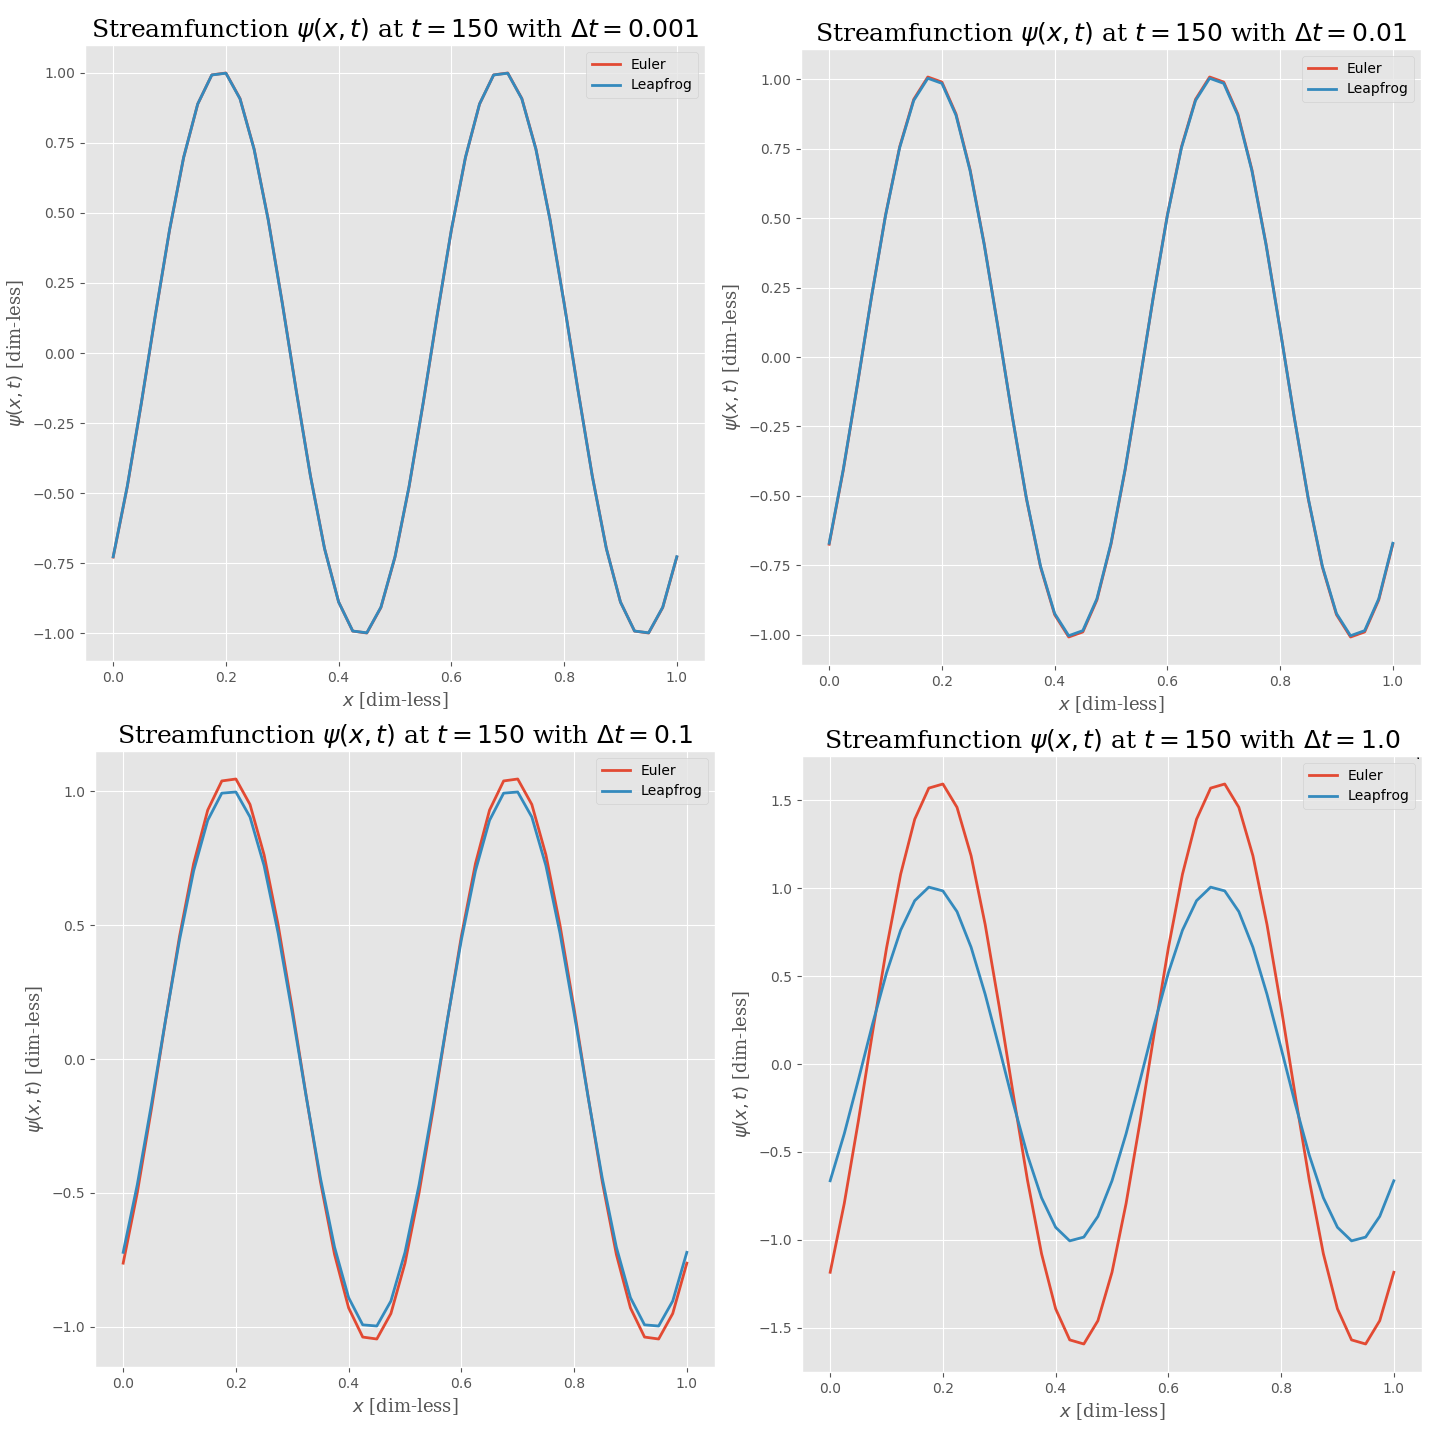
\includegraphics[scale = 0.37]{psi_1d_dt_combined.png}}
 \caption{Figure shows the streamfunction at a time 150 for both the forward Euler scheme and leapfrog scheme. $\Delta t$ is varied while $\Delta x$ is kept constant at 0.025 in the four subplots to attempt to analyze the stability of the two schemes.}
 \label{fig:combi_dt}
\end{figure}


\noindent From figure \ref{fig:combi_dt} we see that the waves have propagated to slightly different positions at a time 150 in the four subplots. This is likely because we write to file at slightly different times for the different values of $\Delta t$ and therefore the streamfunction is at slightly different positions in the four subplots. \\


 %Figure template
\begin{figure}[ht]
 \centerline{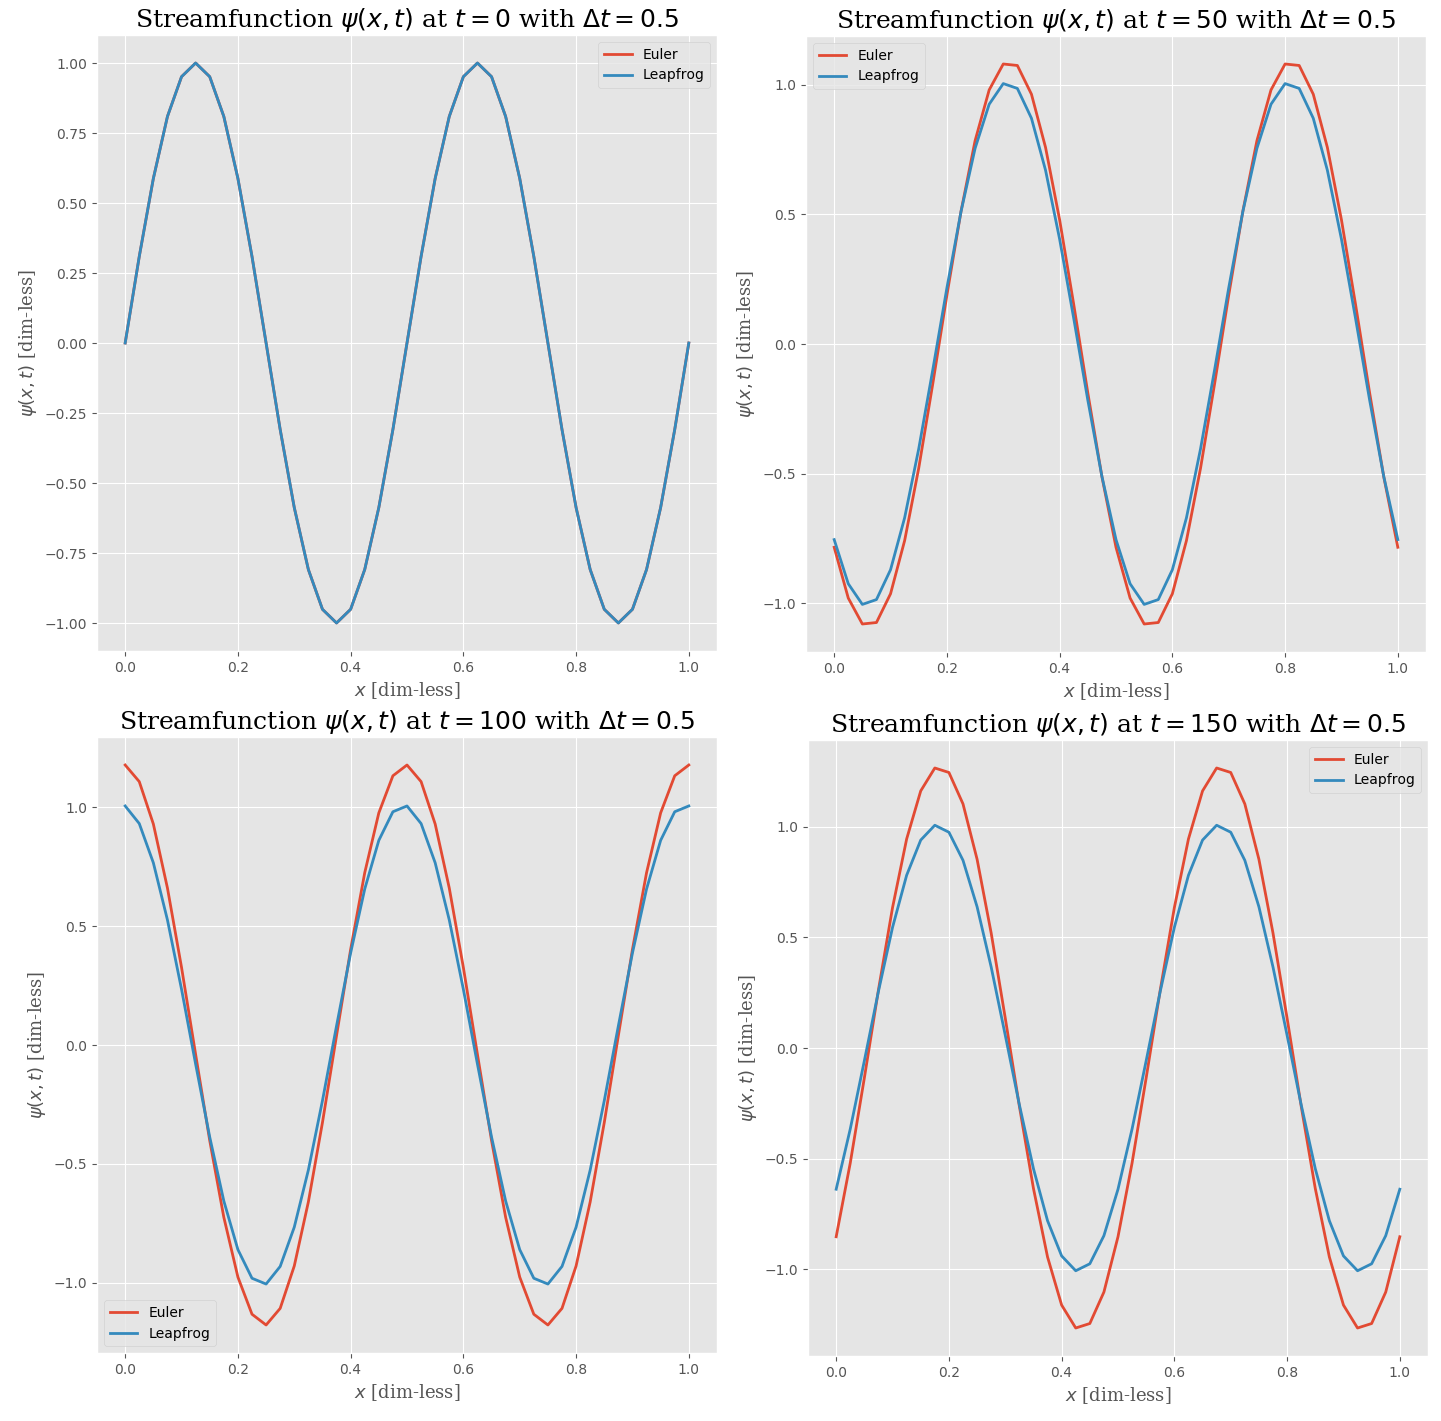
\includegraphics[scale = 0.35]{psi_1d_T_combined.png}}
 \caption{Figure shows the streamfunction for both the forward Euler and leapfrog scheme at four different times, namely 0, 50, 100 and 150. Here we have use a $\Delta t$ of 0.5 and initial streamfunction utilized is $\psi(x,0) = \sin(4 \pi x)$ giving us initial vorticity of $\zeta(x,0) = -16 \pi^2 \sin(4 \pi x)$. Here we can see that the numerical instability in the forward Euler scheme grows progressively as time increases from the initial time 0 to the final time 150.}
 \label{fig:combi_T}
\end{figure}

\noindent In \ref{fig:combi_T} we have examined how the instability of the two schemes develop as a function of simulation time. Here $\Delta t$ is kept fixed and we vary the simulation time for each plot. Also here it is evident that the Euler scheme develops instabilities to a much higher degree than the leapfrog scheme (not at all for these parameters). From both figure \ref{fig:combi_dt} and \ref{fig:combi_T} we can see that the leapfrog scheme is superior in performance compared to the forward Euler scheme. We see that the forward Euler scheme is unstable for different choices of $\Delta t$ and that the instability grows as time elapses. This lead us to the decision to move forward in the project by only utilizing the leapfrog scheme. A great additional benefit, as discused in section \ref{sec:methods}, is that the leapfrog scheme has a lower mathematical truncation error, i.e. is second order accurate in time while the Euler scheme is only first order accurate in time. The only drawback with this scheme is to find the initial $\zeta_j^1$ as discussed in section \ref{sec:implementation_details} and that we have to store the solution at three different time steps when we numerically solve the system of equations given in \eqref{eq:poisson_1d} and \eqref{eq:zeta_eq_1d} compared to at only two times for the forward Euler scheme. This is because we need to always be able to leap over one time step when utilizing the leap frog scheme. So technically, the only downside is slightly more cumbersome implementation and slightly higher memory usage. \\
 

%DISCUSS CHOICE OF $\Delta t$ 
\noindent Now we turn our attention to the choice of $\Delta t$ for the simulations behind the results presented below. Here we need to find a $\Delta t$ which is a good match between both the use of CPU time and numerical precision. We also want our $\Delta t$ set so that the relation in equation \eqref{eq:stability_crit} is exactly fulfilled, with $ |u_0| $ equal to 1, meaning that with a choice of $\Delta x=1/40=0.025$, $\Delta t$ is set to 0.025 as well. This is done to avoid numerical dissipation which can arise when $\Delta t$ becomes very small \cite{lars_petter}. However, we still don't know if this is the exact stability criteria, but during our experimentation, these values for $\Delta t$ and $\Delta x$ seem to work reasnoably well for the leapfrog scheme.\\

%All the links to animations
%1D:
%- Periodic sin(4*pi*x) wave: https://streamable.com/4lpqq
%- Periodic gaussian(sigma = 0.1): https://streamable.com/vds9u

%- Basin  sin(4*pi*x)wave: https://streamable.com/vwmat
%- Basin gaussian(sigma = 0.1): https://streamable.com/n622a
%- Basin gaussian (sigma = 0.25): https://streamable.com/pui15

%2D:
%- Periodic  sin(4*pi*x)wave: https://streamable.com/5u1hq
%- Basin sin(pi*y)*sin(4*pi*x): https://streamable.com/65ypk


\subsubsection{The periodic domain}
%-----------------------------------------------------------------------------------

\noindent We now investigate numerical solutions in the periodic domain. Here we will look at both a sine wave given as \eqref{eq:sine_wave} and a Gaussian wave given as \eqref{eq:gaussian_wave} as initial conditions. \\  

\begin{equation}
		\psi(x,0) = \sin(4\pi x)
        \label{eq:sine_wave}
\end{equation}

\begin{equation}
		\psi(x,0) = e^{- (\frac{x - x_0}{\sigma})^2}
        \label{eq:gaussian_wave}
\end{equation}



\noindent We investigate how our numerical solution behaves in the periodic domain by only utilizing the stable leapfrog scheme. We have used a $\Delta t = \Delta x = 0.025$ and let the simulation run until $t=T=200$. To visualize these results we have, amongst more, made two animations, which for the initial sine wave can be found at \url{https://streamable.com/4lpqq} and the initial Gaussian wave can be found at \url{https://streamable.com/vds9u}. \\

\noindent For the sine wave we see that the wave behaves as expected, it propagates in the negative $x$-direction meaning that the wave moves from east to west as expected (and as predicted by the negative analytical wave speed in section \ref{sec:analytical_periodic}), and as the wave meets the boundary it comes out on the other side as it should when dealing with periodic boundary conditions. The time evolution of $\psi$ also coincides very well with the theoretical prediction made in section \ref{sec:analytical_periodic}. Plotting the analytical solution \eqref{eq:wave_periodic} shows a similar time evolution. \\


\noindent For the Gaussian wave the story is more complicated. Its behavior and wave form gets more messy as time elapses but we can see that the waves are propagating towards the West as expected and that the periodic boundary condition is fulfilled throughout the simulation. We do not have any analytical solutions for the Gaussian initial condition, but we talk more about it's time evolution below.\\ 



\noindent In section \ref{sec:analytical_periodic} we found an analytical expression for the phase speed in a periodic domain as given in equation \eqref{eq:phase_speed_periodic}. Now we wish to see how this compares with our numerical solutions. For this we have made two Hovmuller diagrams, which are shown in figure \ref{fig:hovmuller_periodic} where the diagram to the left and right represent the initial condition of a sine and Gaussian wave respectively. From the Hovmuller diagram it is possible to extract the phase speed as the slope of the time evolution of of some position (e.g. a crest or trough) of the wave. This simply comes from the fact that the time-derivative of position, is velocity.\\ 



%Figure template
\begin{figure}[ht]
 \centerline{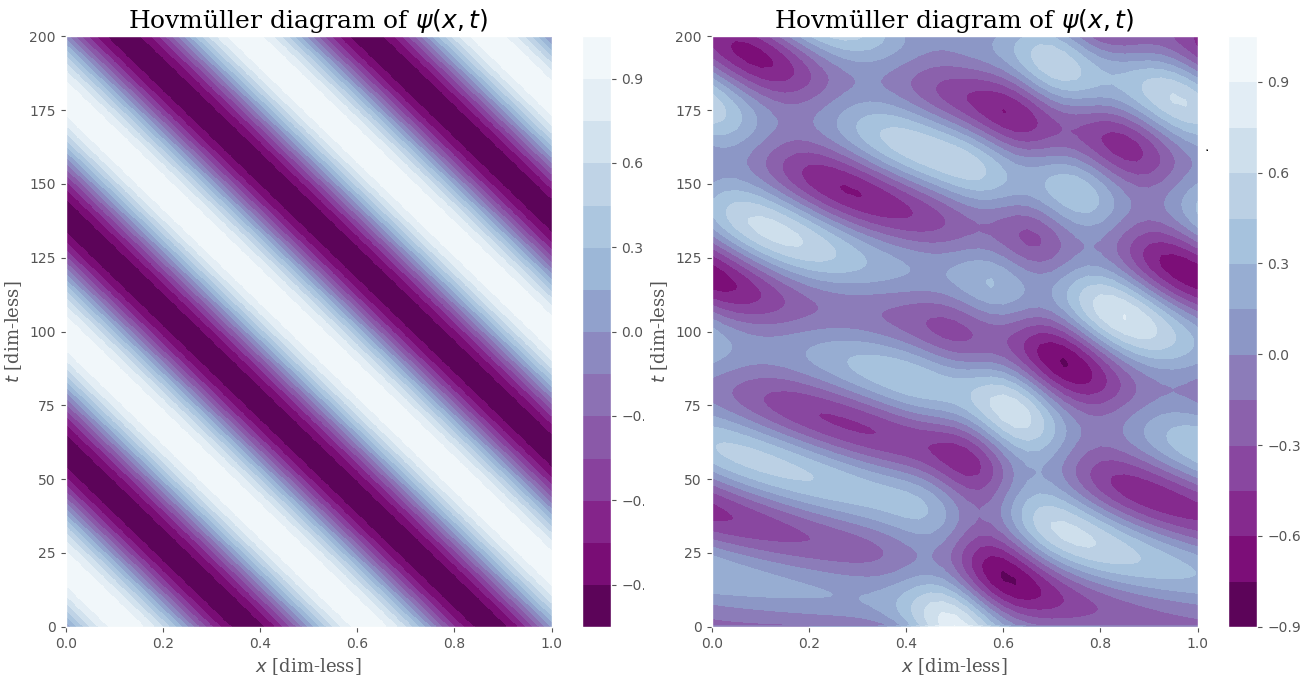
\includegraphics[scale = 0.45]{hovmuller_periodic_combined.png}}
 \caption{The figure shows the Hovmuller diagrams for a simulation of an initial sine and Gaussian wave in a periodic domain to the left and right respectively. }
 \label{fig:hovmuller_periodic}
\end{figure}

\noindent To compare the numerical and analytical phase speed we need to make the terms in equation \eqref{eq:phase_speed_periodic} the same as we have utilized in our numerical simulation, i.e. non-dimensional. For this we set $\beta=1$, $L=1$, $n=2$ and thus the wave number $k$ becomes $4\pi$. This gives the analytical phase speed in the periodic domain to be $-6.33257\times \num{e-3}$. Then we extract the numerical solutions for the phase speed. For the initial sine wave we find, from the Hovmuller diagram to the left in figure \ref{fig:hovmuller_periodic}, that the slope, and thus the phase speed, to be to be $-6.33267 \times \num{e-3}$ through averaging three read offs listed in table \ref{tab:sin_phase}. This is in excellent correlation with the value found analytically for a periodic domain and provides confidence in the numerical solution.\\

\begin{table}[ht]
\begin{center}
\caption{Table lists the phase speed in the periodic domain as found through the left Hovemuller diagram in figure \ref{fig:hovmuller_periodic}.}
  \begin{tabular}{| l | l | l |}
  \hline
    Time &  Position & Slope \\ \hline\hline
     63 & 0.4 & $6.349\times \num{e-3}$ \\
      100 & 0.63 & $6.300\times \num{e-3}$ \\
     126 & 0.8 & $6.349\times \num{e-3}$ \\ \hline
  \end{tabular}
\end{center}
\label{tab:sin_phase}
\end{table}

%Can you find a phase speed?
\noindent As mentioned above regarding the animation for the Gaussian initial condition, we see also in the Hovmuller diagram (right panel in \ref{fig:hovmuller_periodic}) that the motion is far messier. The phase speed for the Gaussian wave initial condition, is not as straight forward to extract from the Hovmuller diagram as for the sine wave. A Gaussian wave can be represented as a sum of sine and cosine terms with different wavenumbers (fourier series) and since Rossby waves are dispersive as seen in section \ref{sec:analytical_periodic}, we thus get waves with different phase speeds, i.e. the initial Gaussian breaks up into several waves with different speeds. It is therefore difficult to extract only one phase speed for the Gaussian case in the Hovmuller diagram. It is also not straight forward to compare the analytical phase speed found analytical in section \ref{sec:analytical_periodic} since this expression is found by the use of a planar wave and extracting wavenumbers for each of the smaller waves is not trivial. \\


%Try varying sigma and see how this affect the phase speed..
\noindent To see how the width of the Gaussian wave affects the phase speed we have varied the value for $\sigma$ and found that increasing $\sigma$ seem to give an increase in the phase speed. This is because when $\sigma$ increases the wavelength increases and thereby the wavenumber $k$ decreases which leads to a larger phase speed in accordance with the dispersion relation. However this was not a very clear finding and we choose only to mention it briefly here. \\





\subsubsection{The bounded domain}
%-----------------------------------------------------------------------------------


\noindent The time has come to investigate how our numerical solutions behave in the bounded domain with solid walls. Here we have imposed the same initial waves as in the periodic domain, both a Gaussian and a sine wave. We have used $\Delta t$ equal to $\Delta x$ equal to 0.025 and the simulation is run up to a time of 200. \\ 

\noindent For the sine wave initial condition we have made a animation which can be found at \url{https://streamable.com/vwmat}. Here we see that the evolution of the wave is the same as we saw in the periodic domain but in addition to what we saw earlier the wave has a modulation which lifts the sine wave up and down in the plane perpendicular to its propagation. If we compare this with the theoretical predictions made in section \ref{sec:analytical_bounded} about the wave solution, we see that the sine factor in \eqref{wave_final} represents a space-dependent amplitude and is responsible for lifting the wave up and down in the plane perpendicular to propagation. We have investigated the analytical solution \eqref{wave_final} graphically and the time evolutions is similar to that of the provided animation.\\

\noindent For the initial condition of a Gaussian wave we have utilized two different widths by setting $\sigma$ equal to 0.1 and 0.25. The two resulting animations can be found at \url{https://streamable.com/n622a} and \url{https://streamable.com/pui15} respectively. Here we can see that the wider wave behave in a more predictable manner as opposed to its thinner more erratic counterpart.\\

%HOW DOES THE MOTION OF GAUSS COMPARE TO SIN IN SAME DOMAIN
\noindent If we compare the behavior of the Gaussian and sine waves in the bounded domain we see that the wave form is quite different and that the evolution of the sine wave is far more predictable than the Gaussian waves. But we also see that the same lifting of the wave in the plane perpendicular to plane of propagation is observed for all initial waves. In other words, the boundary condition of $\psi$ having to be zero at the end points really puts a significant constraint on the solution and the resulting wave is highly affected by this. Another example of how solutions to partial differential equations to do not only depend on the equations itself, but also strongly on the boundary conditions (and initial condition).\\ 

\begin{figure}[ht!]
 \centerline{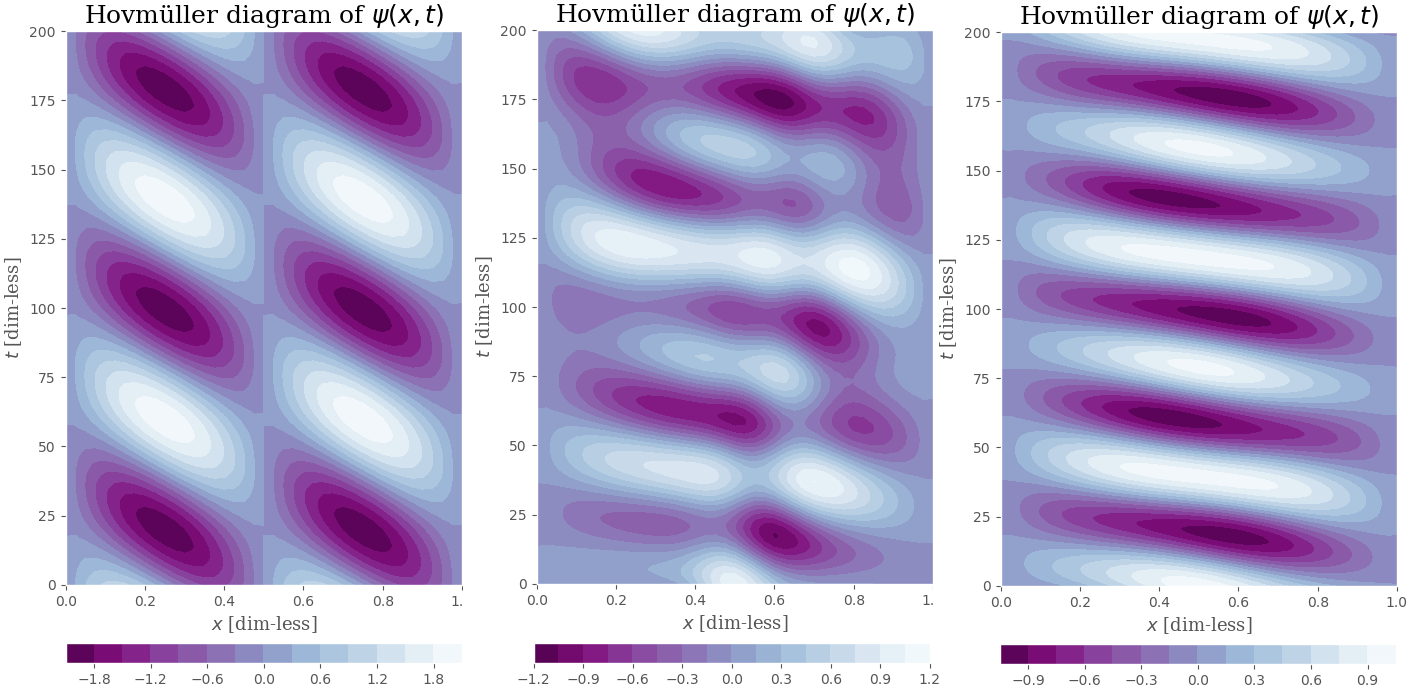
\includegraphics[scale = 0.40]{hovmuller_basin_combined_2.png}}
 \caption{The figure shows three Hovemuller diagram when using initial condition of a sine wave to the left, two Gaussians with $\sigma$ equal to 0.1 and 0.25 in the middle and to the right respectively.}
 \label{fig:hovmuller_bassin}
\end{figure}



\noindent From the Hovmuller diagram presented in figure \ref{fig:hovmuller_bassin} (left: sine, middle: $\sigma=0.1$, right: $\sigma=0.25$) we see, from the two diagrams for the Gaussian initial wave, that phase speed indeed seems to be affected by the width (value of $\sigma$) of the initial wave. As for the periodic case, it is however not easy to extract phase speeds for the initial Gaussian. It is, however, a bit clearer for the wider Gaussian (right). Looking at the slopes, the wider Gaussian seems to produce waves with slightly higher phase speeds seen in the (messy) slopes for the somewhat narrower Gaussian (middle). This can be linked back to the discussion on the periodic domain; a wider initial Gaussian seem to result in propagating waves with larger wavelengths (smaller wavenumbers) and then higher phase speeds.

%-----------------------------------------------------------------------------------
%-----------------------------------------------------------------------------------
\subsection{The 2+1 dimensional system} \label{sec:results_2d}
Then we move on to look at the system in two dimensions. For this case, we have utilized the stable time-stepping scheme, namely the leapfrog scheme, and not looked at the unstable forward Euler scheme. The parameter $\Delta x$ is set equal to $\Delta y$ at 0.025 and $\Delta t=0.01$ was used, and the simulation run up to a time of 200. The reason for the smaller chosen time step than in the 1D case comes from the authors prior experiences where 2D schemes tend to result in slightly stricter stability criteria. We have chosen to use sine waves as initial conditions for our 2D numerical solutions and imposed both periodic and basin boundary condition. \\



\subsubsection{The periodic domain}
%-----------------------------------------------------------------------------------
\begin{figure}[ht]
 \centerline{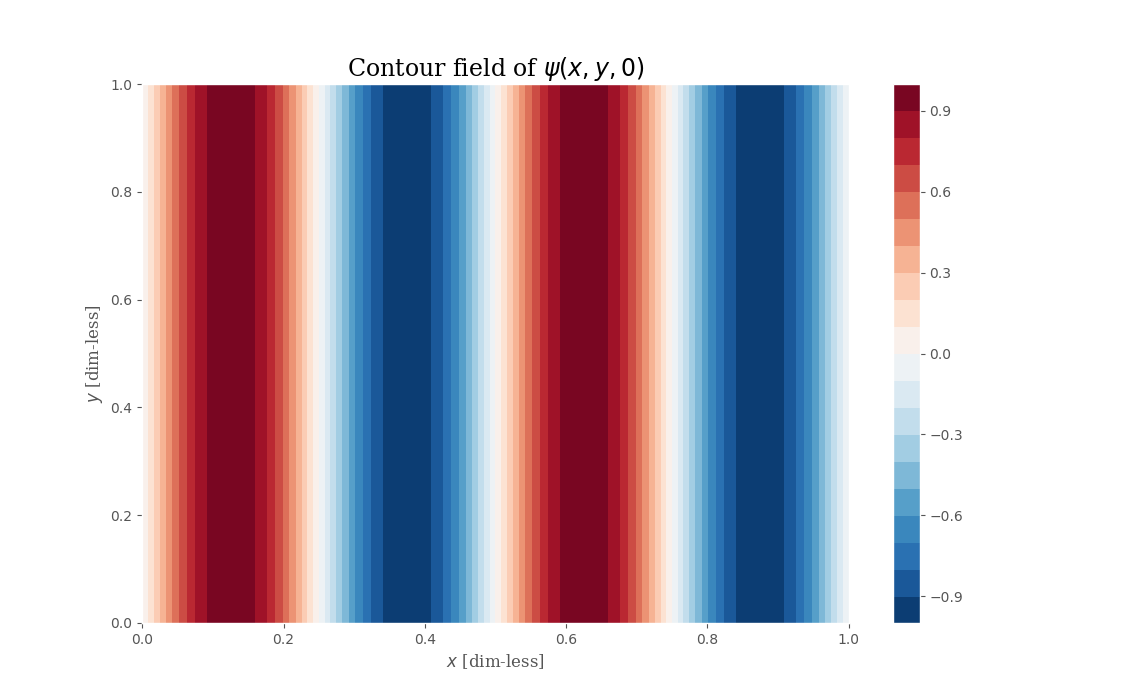
\includegraphics[scale = 0.50]{psi0_2d_periodic.png}}
 \caption{Figure shows the initial sine wave condition, $\psi_0$, utilized for the periodic domain in our 2D case.}
 \label{fig:2d_periodic}
\end{figure}


\noindent We have chosen to use an initial sine wave in the periodic domain given as $\psi(x,y,0) = \sin(4 \pi x)$ as an attempt to verify our 2D solution by the the corresponding solution in the 1D case. Specifically, we wanted to use this initial condition to help us see that our 2D code was working properly. The idea, as elaborated on below, is that the "1D" sine wave initial condition really is a 1D problem that in this case gets extended to 2D. This gives us good intuitive ground for comparison with the 1D solution discussed above. The initial streamfunction used is pictured in figure \ref{fig:2d_periodic} and our resulting time-space evolution can be found at \url{https://streamable.com/5u1hq}. From this we can see that the solution found in our 1D case corresponds well with the 2D version of the problem. Its added dimensionality means the "1D" sine wave expands in "layers" in the $y$-direction (north-south). If we cut our domain horizontally along a specific $y$-value we come back to the solution we found in the corresponding 1D case. We can also see that the periodic boundary condition is obeyed throughout our simulation. We may also notice that the waves have negative phase speeds in the $x$-direction, consistent with earlier theory. It is also worth mentioning that this case could not have been studied in the 2D bounded domain as the "1D" initial sine wave violates the boundary conditions \eqref{eq:dirichlet_bc_2d}, in particular the streamfunction is not zero at the north and south walls with this initial condition.\\

\noindent We also tried to examine the stability of the 2D leapfrog scheme for different choices of $\Delta t$ and $\Delta x$. We used the periodic domain and, but it was difficult to find a conclusive answer for exactly when the solution became unstable, however we did observe that it in fact went unstable for larger values of $\Delta t$. This showed us that the leapfrog scheme is definitely not unconditionally stable and that one also should take care when choosing $\Delta t$ and $\Delta x$ for this scheme.



\subsubsection{The bounded domain}
%-----------------------------------------------------------------------------------
\noindent To investigate how our numerical solution behaves in the 2D bounded domain we have utilized an initial sine wave with an added factor to ensure that the boundary condition is fulfilled in all spatial directions. This gives us the initial wave on the form:

\begin{eqnarray}
	\psi (x,y,0) = \sin(\pi y) \sin(4 \pi x)
    \label{eq:psi_init_2D_bassin}
\end{eqnarray}

\noindent Here the first sine term is added to the streamfunction to ensure that the boundary condition is fulfilled along the border in the $y$-direction as well as in the $x$-direction. The resulting initial wave form can be seen in figure \ref{fig:2d_bassin} and the corresponding animation can be found at \url{https://streamable.com/65ypk}.

\begin{figure}[ht!]
 \centerline{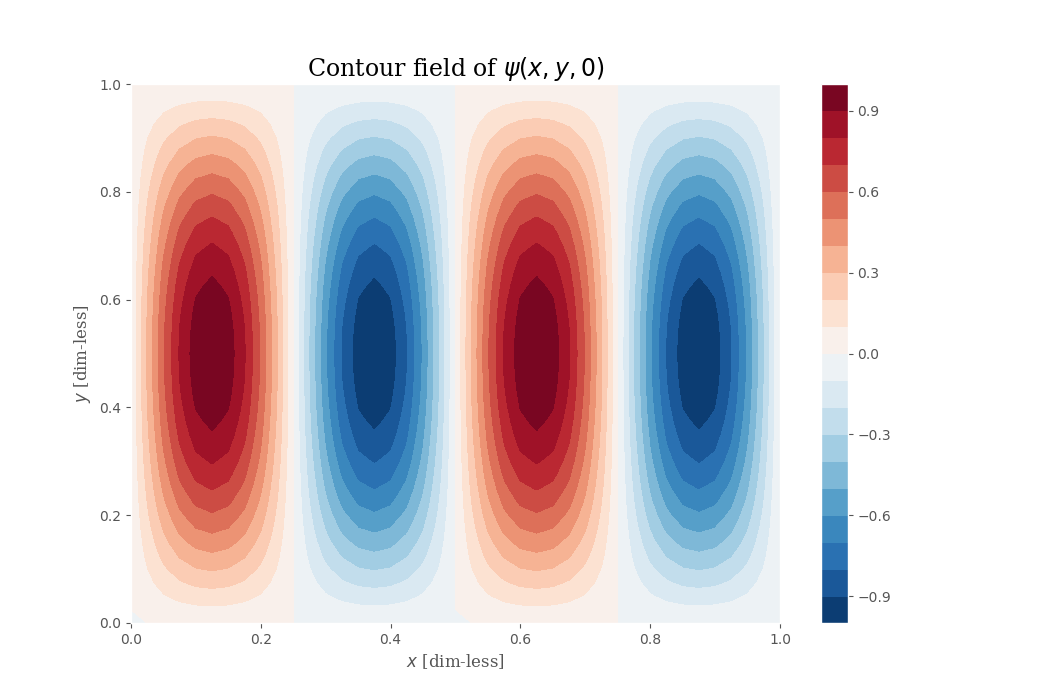
\includegraphics[scale = 0.50]{psi0_2d_basin.png}}
 \caption{Figure shows the initial $\psi$ as given in equation \eqref{eq:psi_init_2D_bassin} utilized in a bounded domain.}
 \label{fig:2d_bassin}
\end{figure}

\noindent First of all we may note that the waves are also here propagating in the negative $x$-direction (west), which is promising considering theoretical predictions in section \ref{sec:analytical_bounded}. Furthermore we can see that the boundary condition is fulfilled for the initial condition as well as throughout our simulations by always being zero at all the boundaries. The added sine term does not only ensure that the boundary condition is fulfilled in the $y$-direction but it also seems to modulate the whole wave, lifting it up and down in the plane perpendicular to its propagation which is the same as we have seen earlier in our bounded domain in 1D. Thus, the phenomena of a present space-dependent wave amplitude, as seen in section \ref{sec:analytical_bounded} (equation \eqref{wave_final}, in order to satisfy the boundary conditions (in the bounded domain) seems to occur also in two dimensions. This seems intuitive and expected. However, there is one noticeable difference; although the whole streamfunction is "lifted" up and down (as in the 1D case), different parts of the field seem to be "lifted" at slightly different times creating some asymmetry between the western and eastern part of the basin. This is in counterpart to the 1D case where the "lifting" occurred equally over the whole domain. The reason behind this is not clear to us, but it could be caused by the initial condition (which is not exactly the same as in 1D) with the additional $\sin(\pi y)$ factor. \\








%====================================================================================
%====================================================================================
\section{Concluding remarks}

\noindent Rossby waves are huge waves propagating horizontally in the atmosphere and ocean which, due to their small vertical displacement and long time scales, are hard to detect. Even though you need satellite radar altimetry to actually observe them, their massive lengths scale causes changes to the Earth's climate condition, even contributing to the effect of El Ni\~no and causing high tides and floods in certain regions of the world \cite{Rossby}. If one wishes to understand and predict these climate conditions, it is also necessary to understand the movement of a Rossby wave and how they propagate information in the atmosphere and oceans.\\

\noindent Solving for the motion of a wave is of course a quite complex task, as the motion is governed by partial differential equations. In this project we used finite difference methods to discretize the equations, and used the Forward-Euler and the leapfrog scheme to advance the equations in time. We then used the Thomas algorithm to repeatedly solve the resulting Poisson equation in one-dimension, and the iterative Jacobi method in two dimensions.\\

\noindent Figure \ref{fig:combi_dt} and figure \ref{fig:combi_T} clearly show that the leapfrog scheme is more stable than the Forward-Euler scheme, and therefore preferable. Both figures also display a sinusoidal form of the wave, which is as predicted by our analytical solutions in section \ref{sec:analytical_periodic}. Table \ref{tab:sin_phase} also strengthens our belief in our numerical solution, as the correspondence between the numerical phase speed and the analytically predicted one is almost suspiciously good. Finally figure \ref{fig:2d_periodic} shows that the wave propagates as expected in two spatial dimensions also, leading us to conclude that our numerical solution quite accurately simulates the propagation of the wave.\\

\noindent In this project we neglected the curvature of the Earth. If one were to proceed with this project, it would be highly interesting to include the curvature of the Earth in our calculations and perhaps make a plot of the Rossby waves across the whole planet to compare with the satellite images mentioned in the introduction \ref{sec:intro}. However this might be a massive task and one might need to consider spherical coordinates or sophisticated projection techniques going from a Cartesian system down onto a sphere. Furthermore it would be interesting to look more at the actual flow field in these simulations. Since we from before have that
\begin{eqnarray}
	u(x,y,t)=-\frac{\partial\psi}{\partial y} \qquad\text{and}\qquad v(x,y,t)=\frac{\partial\psi}{\partial x}
\end{eqnarray}
we would have liked to plot the velocity field together with the $\psi$ field (which is related to the fluid pressure). Assuming northern hemisphere, we could then (hopefully) observe anti-clockwise flow around regions of low pressure (small $\psi$) and clockwise flow around regions of high pressure (larger $\psi$) which would be in correspondence with the very important "geostrophic balance" in geophysical fluid dynamics. Even more accessible could be to look at the time-space evolution of the vorticity $\zeta$ which we actually have  available directly in our simulations.

\pagebreak
%====================================================================================
%====================================================================================


\bibliography{sample}{}
\bibliographystyle{plain}

\end{document}